\section{Лекция 1. Введение в математическую оптимизацию}
\subsection{Содержание курса}
\begin{enumerate}
\item Оптимизация без дополнительных условий (ограничений)
\item Выпуклые множества и конусы
\item Условия оптимальности для выпуклых задач
\item Двойственность и коническая оптимизация
\item Полиномиальные методы выпуклой оптимизации
\item Геометрия линейной оптимизации
\item Симплекс-метод
\item Целочисленная и комбинаторная оптимизация
\end{enumerate}
\newpage
\begin{large}
Глава 1. Оптимизация без дополнительных условий (ограничений)
\end{large}
\vspace{.5 cm}
\begin{center}
\textbf{Структура лекции}
\end{center}

\begin{enumerate}
\item{Функции многих переменных
\begin{enumerate}
\item Отображение
\item Глобальный и локальный экстремум
\item Выпуклые и вогнутые функции
\end{enumerate}
}
\item{Дифференцируемые функции
\begin{enumerate}
\item Производные первого порядка
\item Производные второго порядка
\item Квадратичные функции. Определение матрицы
\end{enumerate}
}
\item{ Критерий оптимальности для дифференцируемых функций
\begin{enumerate}
\item Необходимые критерии
\item Достаточные критерии
\end{enumerate}
}
\item Метод Ньютона
\end{enumerate}
\newpage
\subsection{Обозначения}
Задача оптимизации: $\min\left\lbrace f(x)|x\in X\right\rbrace$ или $\max\left\lbrace f(x)|x\in X\right\rbrace$.\\
(Не обязательно может быть принято.)\\
Написание: $\min{f(x)}$ $\max{f(x)}$, где $x\in X$.\\
$X\subseteq \mathbb{R}^{n} (n\geq 1)$ : Область допустимых значений (область определения).\\
Целевая функция: $f: X\rightarrow \mathbb{R}\cup\left\lbrace -\infty,\infty \right\rbrace$\\
Оптимальное значение: $\inf\left\lbrace f(x)|x\in X\right\rbrace$ или $\sup\left\lbrace f(x)|x\in X\right\rbrace$ (из $\mathbb{R}\cup\left\lbrace -\infty,\infty \right\rbrace$)
\\
Оптимальное решение (оптимальная величина):\\
$x^{*}\in X$, $f(x)=$ Опт.Величина, т.е.
$ f(x^{*})\leq f(x)$ или $ f(x^{*})\geq f(x)$ для всех $x\in X$\\
Недопустимая задача оптимизации: $X=\varnothing$.\\

Неограниченная задача оптимизации: Оптимальное значение $=+\infty$ или $=-\infty$.
\\
(В частности, неограниченная задача допустима).\\
\textbf{Определение 1.1} График функции – это такая область, что $\left\lbrace (x,f(x))|x\in X\right\rbrace \subset R^{n+1}$.\\
\textbf{Определение 1.2} Поверхность уровня (линии уровня для n=2) функции $f$ для величины (значения) $a$ – это такая область, что $\left\lbrace x\in X | f(x)=a \right\rbrace \subset \mathbb{R}^{n}$\\
\textbf{Определение 1.3} Функция $f$ принимает в точке $x^{*}$ свой глобальный минимум на $X$, если условие $f(x^{*})\leq f(x) $ выполняется для всех $ x\in X$.
\begin{itemize}
\item Минимум часто называют глобальным минимумом.
\item Оптимальное решение для $\min\left\lbrace f(x)|x\in X\right\rbrace$ – это в точности те точки, в которых функция принимает свое минимальное значение на  области $X$.
\item Функция может принимать минимальное значение в бесконечном числе точек (например, постоянная функция – константа или $f(x_1,x_2)=\cos(x_1)\sin(x_2)$)
\item Функция может также и вовсе не принимать свое минимальное значение (например, постоянная линейная функция)
\end{itemize}
\textbf{Определение 1.4} Функция принимает в $x^{*}\in X$ свое (локальное) минимальное значение, если $\exists \varepsilon >0$, что $f(x^{*})\leq f(x)$ , $\forall x\in X$ что $\| x-x^{*}\|<\varepsilon$.
\begin{itemize}
\item Глобальный минимум является также и локальным минимумом.
\item Не всякий локальный минимум является глобальным минимумом.
\item Функция может принимать бесконечно много локальных минимумов, либо не принимать их вообще.
\end{itemize}
\textbf{Определение 1.5} Функция называется (строго) выпуклой, если для всех  $x,y \in \mathbb{R}^{n}$ (при $x \neq y$) и $0<\lambda<1$  выполняются условия:
\begin{equation*}
f(\lambda x+(1-\lambda )y)\leq (<) \lambda f(x)+(1-\lambda )f(y)
\end{equation*}
\textbf{Определение 1.6} Функция называется (строго) вогнутой, если для всех  $x,y \in \mathbb{R}^{n}$ (при $x \neq y$) и $0<\lambda<1$  выполняются условия:
\begin{equation*}
f(\lambda x+(1-\lambda )y)\geq (>) \lambda f(x)+(1-\lambda )f(y)
\end{equation*}
\textbf{Наблюдение 1.7} Функция $f$ является выпуклой(вогнутой) тогда и только тогда, когда ее график для всех точек $x,y \in \mathbb{R}^{n}$ лежит под(над) (или возможно на) отрезке, соединяющем две точки $(x,f(x))$ и $(y,f(y))$.\vspace{.1 cm}\\
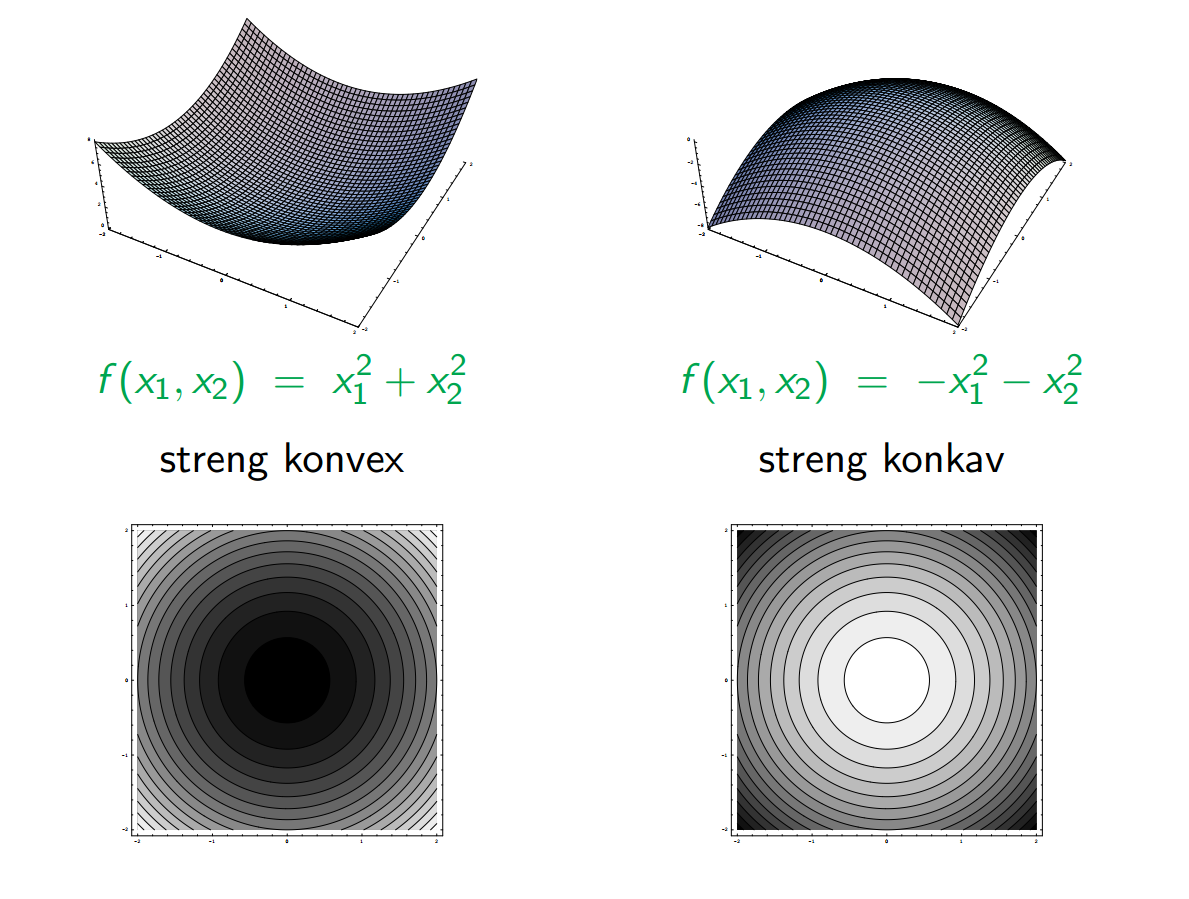
\includegraphics[scale=0.5]{konvex_konkav.png}
\textbf{Предложение 1.8} Если выпуклая(вогнутая) функция принимает в точке значение локального минимума(максимума), то она также принимает значение глобального минимума(максиума) в этой точке.\vspace{.1 cm}\\
\textbf{Замечание 1.9} Если у выпуклой(вогнутой) функции есть глобальный минимум(максимум), то существует единственная (единственно определенная) точка, в которой она его принимает.\vspace{.1 cm}\\
Предложение 1.10 Функция одновременно и выпуклая и вогнутая тогда и только тогда, когда она аффинная.\vspace{.1 cm}\\
\textbf{Определение 1.11} Функция называется аффинной, если она представляется в виде суммы линейной и постоянной функций.\\
$a\in \mathbb{R}^{n}$, $\beta \in \mathbb{R}$:
\begin{equation*}
f(x)=\langle a,x \rangle +\beta
\end{equation*}
для $\forall x \in X$.\vspace{.1 cm}\\
\textbf{Определение 1.12} Скалярным произведением двух векторов $v,w \in \mathbb{R}^{n}$ называется
\begin{equation*}
\langle v,w \rangle=\sum_{i=1}^{n} v_i w_i
\end{equation*}
\textbf{Определение 1.13} Если функция дифференцируема в некоторой точке $x^{*} \in X$, то градиентом этой фунции в точке $x^{*}$ называется
\begin{equation*}
grad_{x^{*}}f:=\left( \frac{\partial f}{\partial x_1}\left( x^{*} \right),\frac{\partial f}{\partial x_2}\left( x^{*} \right),...,\frac{\partial f}{\partial x_n}\left( x^{*} \right) \right)
\end{equation*}
\begin{itemize}
\item Если $v \in \mathbb{R}^{n}$,$\|v\|=1$,то $\langle grad_{x^{*}}f,v \rangle \in \mathbb{R}$--это увеличение (рост) $f$ в точке $х^{*}$ в направлении $v$.
\item ($\|v\|:=\sqrt{\sum_{i=1}^{n}v_{i}^{2}}$ Евклидова норма)
\item Аффинная функция $\varphi(x):=\langle grad_{x^{*}}f,x-x^{*} \rangle +f(x^{*}) $ локально хорошо аппроксимирует (приближает) $f$ в точке $x^{*}$:
\end{itemize}
\begin{equation*}
\lim_{x\rightarrow x^{*}} \frac{f(x)-\varphi(x)}{\|x-x^{*}\|}=0
\end{equation*}
\textbf{Замечание 1.14} Если $f$ дифференцируема в точке $ x^{*} \in int(X)$, $\alpha=f\left(x^{*}\right)$ то $grad_{x^{*}} f$ ортогонален линии уровня функции $f$ с параметром $\alpha$ и показывает направление наибольшего роста функции $f$ в точке $x^{*}$.
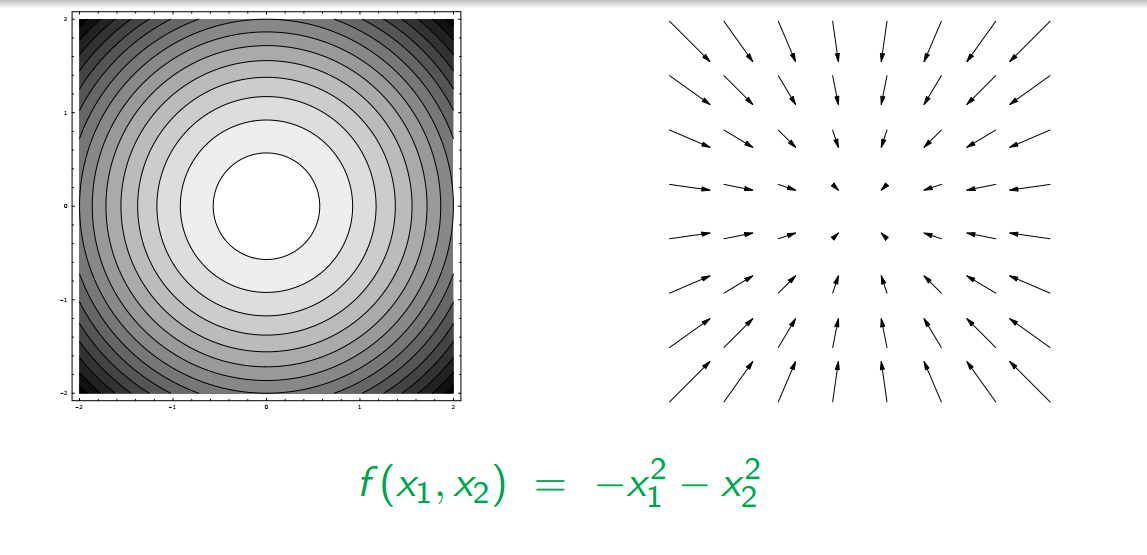
\includegraphics[scale=0.5]{grad.png}
\textbf{Определение 1.15} Если Функция $f$ дважды дифференцируема в точке $x^{*}\in int(X)$, то матрицей Гессе $f$ в точке $ x^{*}$ называется матрица:
\begin{equation*}
hess_{x^{*}}f:=\begin{pmatrix}
 {\frac{\partial^{2} f}{\partial x_1 \partial x_1}(x^{*})}& ...& {\frac{\partial^{2} f}{\partial x_1 \partial x_n}(x^{*})}\\
 ...& ...& ...\\
{\frac{\partial^{2} f}{\partial x_n \partial x_1}(x^{*})}& ...& {\frac{\partial^{2} f}{\partial x_n \partial x_n}(x^{*})}
\end{pmatrix}
\end{equation*}
\begin{itemize}
\item Если $f$ дважды диифференцируема, то матрица $hess_{x^{*}}f$ симметричная.
\item Квадратичная функция $q(x):=\frac{1}{2}(x-x^{*})^{T} \left( hess_{x^{*}} f\right)(x-x^{*})+\left\langle  grad_{x^{*}}f, x- x^{*} \right\rangle +f(x^{*})$ аппроксимирует функцию $f$ локально хорошо в точке $x^{*}$:
\end{itemize}
\begin{equation*}
\lim_{x\rightarrow x^{*}} \frac{f(x)-q(x)}{\|x-x^{*}\|^{2}}=0
\end{equation*}\vspace{0.3 cm}
\subsection{Дополнение: обозначения для матриц и векторов}
\begin{itemize}
\item $\left[ p \right] := \left\lbrace 1,2,...,p \right\rbrace$
\item $\mathbb{R}^{ \left[ m \right] \times \left[ n \right] }$: Область (пространство) действительных матриц  $\left[ m \right] \times \left[ n \right]$.
\item Особые матрицы:  \begin{itemize}
		\item $\mathbb{O}_{p} \in \mathbb{R}^{p}$,$\mathbb{O}_{ \left[ m \right] \times \left[ n \right] }$: нуль-ветор, нуль-матрица.
		\item $\mathbbm{1}_{p} \in \mathbb{R}^{p}$,$\mathbbm{1}_{ \left[ m \right] \times \left[ n \right] }$: единичный вектор, единичная матрица.
		\item $\mathbb{I}_{ \left[ m \right] \times \left[ n \right] }$: матрица инцидентности
		\item Единичный вектор (полагаю замечание относительно контекста имеет отношение к нему)
		\item $\mathbbm{e}_{i}=\left(0,...,0,1,0,...,0 \right)$ : $i$-ый единичный веркор
	   \end{itemize}
\item Для $A \in \mathbb{R}^{ \left[ m \right] \times \left[ n \right] }$, $i \in \left[ m \right]$, $j \in \left[ n \right]$:
	\begin{itemize}
	\item $A_{(i,j)}=A_{ij}=a_{ij}$: значение матрый на $i$ строке, $j$ столбце.
	\item $A_{(i,*)} \in \mathbb{R}^{n}$: $i$-ая строка матрицы $A$
	\item $A_{(*,j)} \in \mathbb{R}^{n}$: $j$-ый столбец матрицы $A$
	\end{itemize}
\item В терминах произведения матриц: отождествление $\mathbb{R}^{p}$ с $\mathbb{R}^{ \left[ p \right] \times \left[ 1 \right]}$ (вектор-столбцы)
\end{itemize}
